\documentclass{article}
\usepackage[main,final]{neurips_2026}
\usepackage[utf8]{inputenc}
\usepackage[T1]{fontenc}
\usepackage{hyperref}
\usepackage{url}
\usepackage{booktabs}
\usepackage{amsmath}
\usepackage{amsfonts}
\usepackage{graphicx}
\usepackage{xcolor}
\usepackage{microtype}

\title{FaceTrap: On-Device Face Recognition with a Target-Conditioned Android Availability Demonstration}

\author{%
  \begin{tabular}{@{}c@{\hspace{2.5cm}}c@{}}
    \textbf{Sudhanva Bharadwaj B. M.} & \textbf{Dhanya V. Koteswari} \\
    CS3B051 & CS23B055 \\
    Dept. of CSE & Dept. of CSE \\
    IIT Tirupati & IIT Tirupati
  \end{tabular}
}

\begin{document}
\maketitle

\begin{abstract}
We present FaceTrap, an Android proof of concept that studies how a face-authentication interface can conceal a target-dependent availability-impact action. Starting from one image for each enrolled identity, a latent-diffusion image-to-image pipeline produced 1,500 synthetic portraits spanning apparent age, illumination, pose, scale, expression, and background. We introduce a deterministic, identity-stratified 80/10/10 split and prevent evaluation leakage by forming ArcFace reference centroids only from the 1,200-image training partition. An SCRFD detector and ArcFace encoder run locally through ONNX Runtime on Android. A logistic calibrator fitted on the 150-image validation partition maps the target cosine score to decision confidence; confidence strictly above 0.85 activates the Android availability demonstration. On the 150-image synthetic test partition, all faces were detected, identity accuracy was 100\%, target precision/recall/F1 were 1.00, and target ROC AUC was 1.00. These results demonstrate internal consistency, not real-world biometric validity: all samples derive from three source identities and a shared generator. In the controlled emulator, the target path records app-private event markers and starts an AES-256-GCM shared-storage processing routine. The interface presents the affected scope, output format, event timer, and manifest. No network communication or persistence mechanism is implemented.
\end{abstract}

\section{Introduction}

Biometric authentication is normally designed to make one visible decision for every user. A compromised implementation could instead expose an ordinary success path to known users while assigning a covert action to one selected identity. The CS402M scenario asks us to demonstrate this risk with severe data scarcity: one input portrait per identity, synthetic generation, a face-authentication application, and a target-dependent ransomware-style effect inside a controlled Android environment.

FaceTrap makes three contributions. First, it defines a reproducible 1,500-image dataset with disjoint train, validation, and test manifests. Second, it combines efficient SCRFD detection~\citep{guo2021scrfd} with 512-dimensional ArcFace embeddings~\citep{deng2019arcface} in a fully on-device Android pipeline. Third, it connects a target-only biometric decision to a controlled Android availability demonstration, maintains an app-private incident record, and communicates the scope and state through a dedicated incident interface.

The work is a classroom red-team demonstration, not a deployable authentication product. Because the current availability path changes eligible files, all development and demonstrations must remain restricted to a dedicated disposable emulator/VM snapshot containing no personal data.

\section{Related work}

ArcFace learns discriminative features on a normalized hypersphere using an additive angular margin~\citep{deng2019arcface}. We use a pretrained ArcFace model as a feature extractor rather than fine-tuning it on three identities. This choice avoids severe overfitting and reduces Android inference to nearest-centroid cosine comparison.

SCRFD reallocates sampling and computation to obtain an efficient face detector suitable for resource-constrained inference~\citep{guo2021scrfd}. Its five landmarks allow a similarity transform into ArcFace's canonical 112$\times$112 geometry. Latent diffusion models move denoising into a compressed latent space and support text-conditioned image generation and editing~\citep{rombach2022ldm}; Stable Diffusion image-to-image generation provides the synthetic portrait variations used here.

Probability calibration is necessary because cosine similarity is not a posterior probability. FaceTrap therefore learns a one-dimensional logistic mapping on validation data and reserves the assignment's 0.85 rule for the calibrated target confidence, rather than incorrectly interpreting raw cosine as probability.

\section{Dataset and reproducibility}

\subsection{Single-image generation}

The dataset contains three identities: two Class A team members (\texttt{you} and \texttt{teammate}) and one Class B target professor. Each identity has exactly 500 PNG images at 512$\times$512 resolution. Stable Diffusion v1.5 image-to-image generation is run locally. For Class A, strength is 0.15; for Class B, strength is 0.20. Both use guidance scale 7.0 and 30 denoising steps. Prompts sample scale, lighting, small pose changes, background, and expression. Apparent-age prompts are enabled for the designated aging sets. A negative prompt suppresses multiple faces, deformation, blur, illustration styles, and extreme poses.

The generator records filename, identity, prompt attributes, and random seed in per-identity CSV metadata. The scripts use local model files and expose the exact prompt vocabularies. This preserves reproducibility while acknowledging that text prompts do not guarantee independent or physically accurate variation.

\subsection{Deterministic split}

\texttt{prepare\_dataset\_splits.py} performs identity-stratified shuffling with seed 402. It writes CSV manifests rather than duplicating 504 MB of images. Table~\ref{tab:splits} gives the resulting counts. An automated overlap check found zero shared paths between partitions and a union of 1,500 unique images.

\begin{table}[t]
  \caption{Deterministic dataset split. Class A combines the two enrolled team members.}
  \label{tab:splits}
  \centering
  \begin{tabular}{lrrrr}
    \toprule
    Split & You & Teammate & Professor & Total \\
    \midrule
    Train & 400 & 400 & 400 & 1,200 \\
    Validation & 50 & 50 & 50 & 150 \\
    Test & 50 & 50 & 50 & 150 \\
    \bottomrule
  \end{tabular}
\end{table}

Splitting individual synthetic outputs does not eliminate source-identity leakage: every partition ultimately derives from the same three reference portraits and generator family. The split prevents direct image reuse, but it is not equivalent to testing on independently captured people or environments.

\section{Method}

\subsection{On-device face recognition}

CameraX supplies the latest frame. SCRFD runs at 640$\times$640 with detection threshold 0.50. The largest detected face is aligned from five landmarks to 112$\times$112. ArcFace produces an L2-normalized vector $e\in\mathbb{R}^{512}$. For identity $i$, the training reference is the normalized centroid
\begin{equation}
  r_i = \frac{\sum_{j=1}^{n_i} e_{ij}}{\left\|\sum_{j=1}^{n_i} e_{ij}\right\|_2},
\end{equation}
where $n_i=400$. The predicted identity maximizes $s_i=e^\top r_i$. Scores below 0.30 are rejected as unknown. Reference embeddings shipped with the app are rebuilt exclusively from the training manifest; validation and test vectors never contribute to them.

\subsection{Target-confidence calibration}

Raw cosine values for the professor were cleanly separated but below 0.85: validation target scores ranged from 0.7011 to 0.8465, whereas non-target professor scores were at most 0.1316. Applying 0.85 directly would therefore yield zero triggers. We fit logistic regression ($C=10$, seed 402) on validation professor scores:
\begin{equation}
  P(B\mid s_B)=\sigma(10.582016s_B-4.672831).
\end{equation}
Path B requires that professor is the best identity and $P(B\mid s_B)>0.85$. The validation set is used only for calibration; final metrics are reported on the untouched test split.

\subsection{Two authentication paths}

For Path A, either enrolled student above the recognition threshold displays ``Authentication successful'' and appends a timestamped internal audit event. For Path B, a professor match above the calibrated confidence threshold initializes the availability demonstration, writes an event manifest, and starts a non-exported full-screen incident activity. The activities and inference run locally. The application requests camera access for recognition and broad storage access for the emulator-only availability path; it declares no network permission.

\subsection{Availability-impact simulator}

The current implementation has two related layers. The app-private layer creates three fictional decoys under \texttt{filesDir/availability\_demo}, writes access and system-state markers, records SHA-256 hashes, identity, calibrated confidence, scope, and timestamp in \texttt{ransomware\_manifest.txt}, and makes its demonstration reader reject decoy access after the trigger. These files support a repeatable event record and do not themselves represent the shared-storage operation. Android documents this app-specific storage as private to the app~\citep{androidstorage}.

The second layer is implemented by \texttt{DataManager}. After storage authorization, it obtains or creates a 256-bit AES key in Android Keystore and asynchronously visits eligible shared-storage files. Each successful operation writes a \texttt{.bak} output containing a 12-byte GCM nonce followed by AES-GCM ciphertext, then removes the source file. It excludes this application's internal files, cache, and package-specific \texttt{Android/data} directory, skips existing \texttt{.bak} outputs and most hidden files, and records processed paths in an internal list. A marker prevents the routine from starting a second time. There is no in-app decrypt/restore workflow; emulator snapshot restoration is therefore the required recovery boundary. In this report, ``simulation'' denotes the controlled disposable-emulator setting and presentation, not an assertion that the cryptographic file operation is virtual.

\subsection{Interface design}

The camera remains full-screen but is now organized as an authentication interface rather than a raw preview: a rounded face guide establishes positioning, top-level chips expose application and system state, and a bottom result panel preserves the live recognition text written by the activity. The incident activity uses a consistent dark visual system and separates five kinds of evidence: target-trigger context, a one-hour visual timer, current system status, storage scope and cryptographic output, and the selectable event manifest. The layout also states that the countdown is visual only. These changes are implemented entirely in Android XML resources; recognition, trigger, storage, and activity logic are unchanged.

\section{Experimental setup}

Evaluation used Ubuntu 22.04, Python 3.10.12, ONNX Runtime's CPU execution provider, and 12 logical CPUs. Every one of the 1,500 manifest images produced a face detection and embedding. The ordinary recognition threshold was 0.30. Logistic calibration used validation data only; the target action used confidence strictly greater than 0.85. Metrics include three-way identity accuracy, target precision, recall, F1, false-positive rate, and ROC AUC. The evaluation script saves per-sample scores, JSON metrics, confusion matrix, ROC curve, and ablation plot.

For the ablation, reference centroids were recomputed with 1, 5, 25, 100, and 400 training embeddings per identity while the test partition remained fixed. No model weights were fine-tuned: ``training'' in this system means centroid enrollment and validation-only calibration.

\section{Results}

\begin{table}[t]
  \caption{Measured validation and held-out synthetic-test performance.}
  \label{tab:metrics}
  \centering
  \begin{tabular}{lcc}
    \toprule
    Metric & Validation & Test \\
    \midrule
    Detected / total & 150/150 & 150/150 \\
    Identity accuracy & 1.000 & 1.000 \\
    Target precision & 1.000 & 1.000 \\
    Target recall & 1.000 & 1.000 \\
    Target F1 & 1.000 & 1.000 \\
    Target false-positive rate & 0.000 & 0.000 \\
    Target ROC AUC & 1.000 & 1.000 \\
    \bottomrule
  \end{tabular}
\end{table}

\begin{figure}[t]
  \centering
  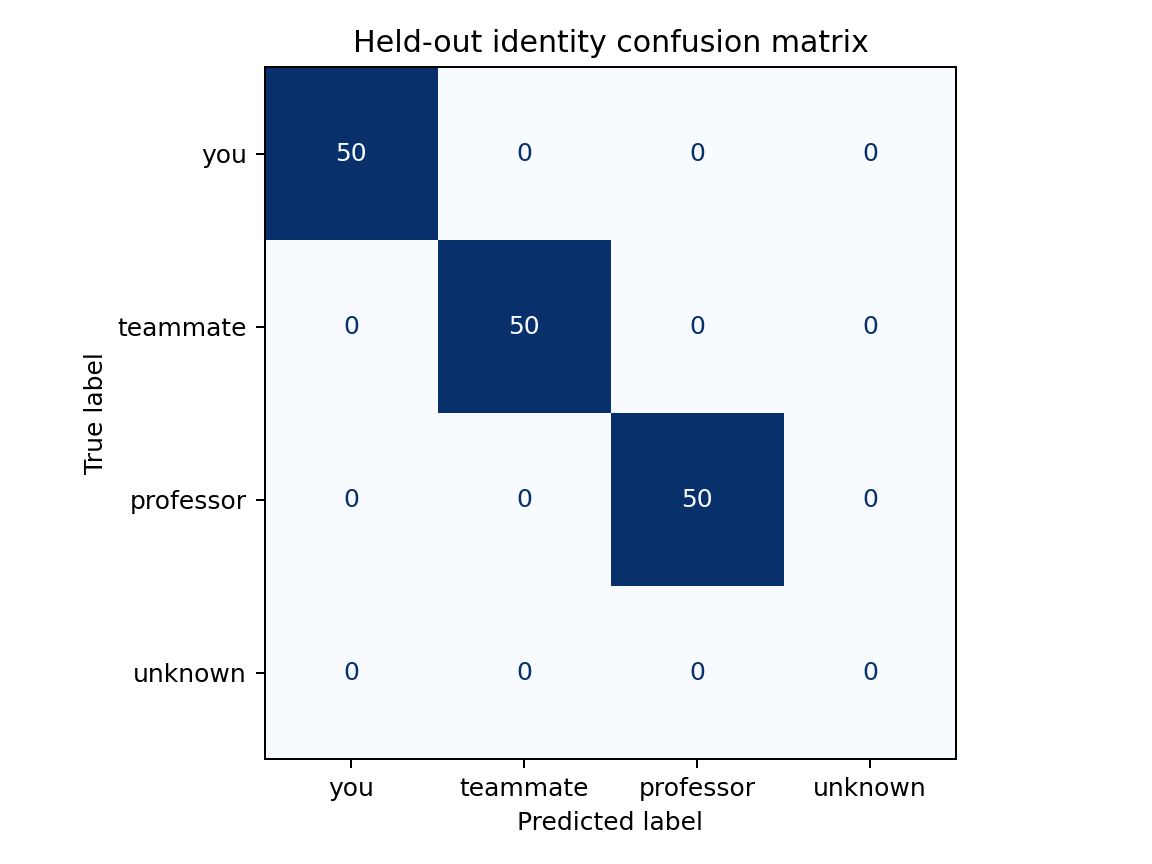
\includegraphics[width=0.47\linewidth]{results/confusion_matrix.png}\hfill
  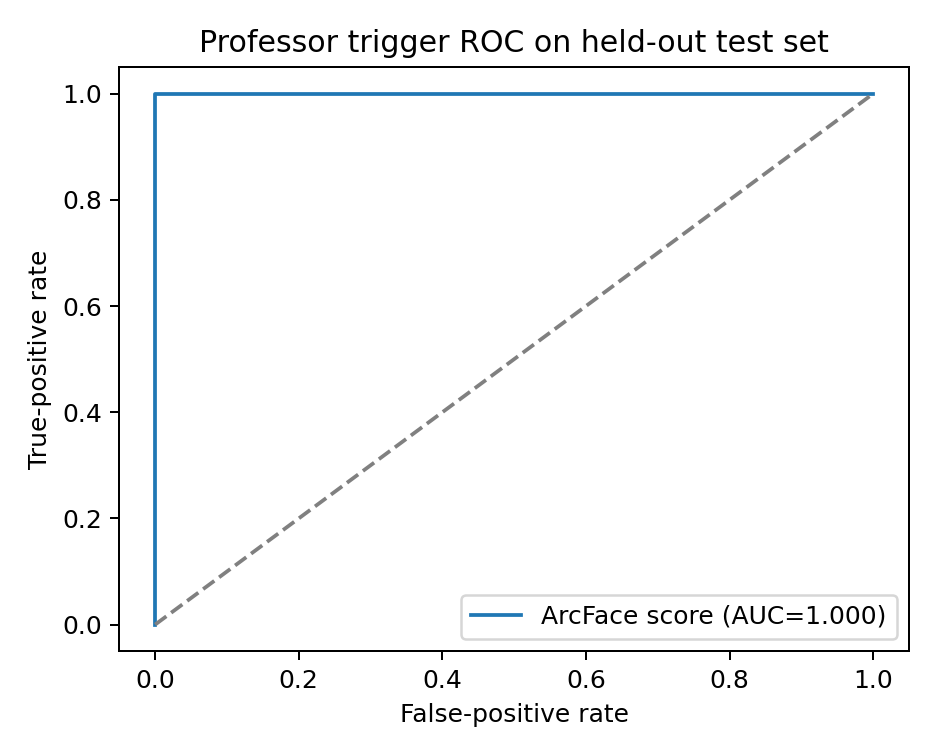
\includegraphics[width=0.47\linewidth]{results/roc_curve.png}
  \caption{Held-out synthetic results. Left: identity confusion matrix. Right: professor-score ROC curve. Perfect separation must be interpreted in light of the shared-source synthetic dataset.}
  \label{fig:results}
\end{figure}

Table~\ref{tab:metrics} and Figure~\ref{fig:results} show perfect separation on the generated holdout. The test target confusion counts were TN=100, FP=0, FN=0, and TP=50. This confirms that the implementation, manifests, centroids, calibration, and trigger logic agree on the present data. It does not justify a claim of perfect face recognition in deployment.

The centroid-size ablation also produced identity accuracy and target AUC of 1.0 for every tested size from 1 to 400 images per identity. Rather than proving that one sample is universally sufficient, this indicates that identity cues shared by generated variants dominate the test split. The flat ablation is evidence of an easy synthetic benchmark and motivates independent real-camera evaluation.

\paragraph{Android emulator verification.} A live run on 23 August 2026 used an x86-64 Android API 36 emulator with the host webcam. CameraX supplied rotated 480$\times$640 analysis frames and the application produced both accepted and unknown decisions. In the witnessed target run, the professor was the best identity at raw cosine 0.7626; calibration mapped this to 0.9676, exceeding the strict 0.85 gate. Path B then recorded the decoy availability state and created the app-private manifest with timestamp, identity, confidence, and hashes. The marker and manifest were independently read with \texttt{adb shell run-as}. This run verified the biometric-to-incident transition and private event record; it did not measure shared-storage throughput, encrypted-file count, or recovery success, so none of those are claimed as experimental results.

\section{Failure modes, limitations, and ethics}

\paragraph{Synthetic distribution shift.} Diffusion outputs may retain source-image background, capture artifacts, and identity shortcuts. Real camera blur, exposure, display moir\'e, masks, extreme pose, and aging can move embeddings outside the observed ranges. The perfect synthetic metrics should therefore be treated as an upper bound on this narrow dataset.

\paragraph{Identity count and fairness.} Only three identities are evaluated, so demographic fairness, open-set behavior, and population-scale false matches cannot be estimated. The app selects the largest detected face; multi-person frames are outside the evaluated scope.

\paragraph{Calibration.} The logistic mapping is fitted to only 150 validation images generated from the same sources. A different camera, generator, or ArcFace model requires recalibration. Calibration changes confidence interpretation but not score ranking.

\paragraph{Presentation attacks.} The assignment demonstration explicitly allows a printed or second-screen target image, so the app intentionally has no liveness detector. It must not be described as secure biometric authentication.

\paragraph{Dual-use risk and safeguards.} Target-conditioned behavior and bulk file transformation are dual use. The interface visibly labels the exercise as a simulation and the application has no network permission, downloader, persistence, or privilege-escalation mechanism. Those properties do not make the storage operation harmless: broad storage authorization and source removal create a real availability impact inside the test device. Accordingly, the APK must be run only on a disposable course emulator/VM with a verified clean snapshot and no personal or connected cloud data. It must not be installed on a personal or production device. Face images and embeddings are biometric data and should be published only with informed consent and course authorization.

\section{Conclusion}

FaceTrap demonstrates how a visually ordinary face-authentication pipeline can contain identity-dependent behavior. Deterministic splitting and train-only enrollment correct the original evaluation leakage risk. Validation calibration makes the required 0.85 confidence gate meaningful for an ArcFace cosine system. Perfect synthetic-test results verify pipeline consistency but reveal the benchmark's limited diversity; real-world robustness, fairness, liveness, and security remain unproven. The Android implementation connects the calibrated target decision to an auditable app-private event record, an emulator-scoped availability operation, and a redesigned incident interface. Its real shared-storage side effects make isolation and snapshot-based recovery mandatory parts of the demonstration protocol.

\bibliographystyle{plainnat}
\bibliography{references}

\appendix
\section{Reproduction commands}

\begin{verbatim}
python3 prepare_dataset_splits.py
python3 -m venv .venv
.venv/bin/pip install -r requirements-evaluation.txt
.venv/bin/python evaluate_face_model.py
python3 -m unittest discover -s tests -v
./gradlew assembleDebug
cd report
pdflatex neurips_2026.tex
bibtex neurips_2026
pdflatex neurips_2026.tex
pdflatex neurips_2026.tex
\end{verbatim}

The evaluation outputs are under \texttt{report/results}. The debug APK assembly is the verified Android build target for this revision. The existing local availability-test fixture still calls an older trigger signature, and Android lint reports a pre-existing API-level guard issue in the storage-permission result callback; neither is counted as passing evidence. Demonstration-video recording, portal upload, and final link submission are assigned to the team separately and are not represented as completed experimental evidence in this report revision.

\section{Team contributions}

\textbf{Sudhanva Bharadwaj B. M. (CS3B051):} primary development of the face-recognition pipeline, including CameraX frame acquisition, SCRFD detection, five-point face alignment, ArcFace ONNX inference, reference-embedding comparison, recognition thresholds, and target-confidence integration; integration and testing of the end-to-end biometric decision flow; report integration and interface refinement.

\textbf{Dhanya V. Koteswari (CS23B055):} primary development of the Android file-encryption/availability simulation, including Android Keystore key handling, AES-256-GCM file processing, operation-state markers, affected-file tracking, and integration of the incident behavior; review of the controlled-emulator demonstration and report.

Both members contributed to integration decisions, final emulator testing, report review, and demonstration preparation. The division above identifies the primary ownership of each technical pipeline.

\section{Generative-AI prompt disclosure}

Generative AI was used as a coding and writing assistant. The two material prompt groups were:
\begin{enumerate}
  \item Analyze the supplied CS402M brief and the teammate-provided reference repository; add a distinct professor-triggered Android sandbox demonstration, implementation notes, tests, and no repository push. The assistant was instructed to be cautious, concise, and not copy the reference project.
  \item Complete the deterministic 80/10/10 dataset split, train-only embedding evaluation, NeurIPS-format report, two-member contribution division, explicit Ubuntu testing instructions, and incorporation of witnessed emulator evidence. Video production and review activities were assigned to the team separately.
\end{enumerate}

AI-produced changes were reviewed against the assignment, compiled, statically scanned, and exercised with automated tests. Metrics in this report were read from \texttt{report/results/metrics.json}; no experimental values were invented. Implementation, verification, and safety decisions are documented in the repository \texttt{README.md}.

\end{document}
